% !TeX root = ../thuthesis-example.tex

\chapter{引言}

随着人脸识别、自然语言处理等人工智能应用使用越来越广泛,各种针对机器学习模型的攻击也层出不穷。
机器学习模型需要使用数据进行训练,一旦模型被攻陷,被用于训练的数据将会有泄漏的风险。
当今人们隐私保护的意识越来越强,并且有关隐私保护的法规也相继出台,面对越来越多针对机器学习模型的攻击我们该如何应对呢呢?
本章将从机器学习模型的攻击,GDPR等隐私法规的出台和卷积神经网络的应用三方面介绍本文的研究背景,最后将介绍本文的选题意义。

\section{研究背景及意义}

\subsection{机器学习模型的攻击}
随着机器学习技术在实际应用中的普及,越来越多针对机器学习模型的攻击也随之产生。
纵观针对机器学习模型的攻击方法,大致可以分为三种攻击类型,分别是模型抽取攻击(Model Extraction Attack)、模型逆向攻击(Model Inversion Attack)还有成员推理攻击(Membership Inference Attack)。
模型抽取攻击是指利用机器学习模型的输出数据,进行分析综合,最终获取模型参数的机器学习模型攻击方法。
模型逆向攻击是指利用机器学习模型的输出数据,进行推理分析,最终推断出重要的统计信息的机器学习模型攻击方法。
成员推断攻击是指利用机器学习模型的输出数据,进行加工统计,最终判断某条记录是否被用于训练目标模型的机器学习模型攻击方法。
三种方法相同点和不同点的对比如表~\ref{tab:model-attack-difference}所示。
\begin{table}
    \centering
    \caption{机器学习模型攻击方法的对比}
    \begin{tabular}{lll}
      \toprule
      攻击类型  & 攻击途径 & 攻击目标  \\
      \midrule
      模型抽取攻击   & 利用模型API输出 & 获取模型 \\
      模型逆向攻击   & 利用模型API输出 & 获取统计信息                    \\
      成员推断攻击 & 利用模型API输出  & 判断某记录是否被用于训练模型  \\
      \bottomrule
    \end{tabular}
    \label{tab:model-attack-difference}
\end{table}

随着越来越多针对机器学习模型攻击的产生,机器学习模型的信息泄露问题应当得到重视。一些用户不希望自己隐私数据被用来训练模型,因此一些已经训练好的模型想办法将这部分用户的数据进行“遗忘”。
\subsection{隐私保护法规的相继出台}
用户的被遗忘权早在2016年就被欧盟在《通用数据保护条例(GDPR)》提出。《通用数据保护条例(GDPR)》\cite{gdpr2018}(以下简称“GDPR”)是由欧盟2016年4月正式提出,并于2018年5月25日正式生效。
GDPR的生效取代了欧盟自1995年实施的《数据保护指令》。与《数据保护指令》相比,GDPR更加注重隐私保护的实施细节,从而更好地保护用户的隐私数据。在GDPR的第三章第17条中提到了“Right To Be Forgotten”。
文章中写道,当用户撤销数据使用授权的时候,数据控制人应当立即删除用户数据以及其拷贝、连接和复制品。这就意味着如果一个公司从一个用户那里获取了一张用户提供的图片用于机器学习,那么当这个用户要求公司遗忘数据时,这个公司应当立即删除用户提供的图片,并且将机器学习模型恢复到没用这张图片学习的状态。
一旦这家公司真的这么做,就会面临一个挑战,那就是要重新训练机器学习模型,这样的代价是非常大的,因为机器学习的训练往往需要很长时间,几个小时、几天甚至几周。
此外,GDPR适用范围是很广的。在第3条适用范围中指出,即使这个公司不在欧盟范围内,只要这家公司向欧盟内公民提供了服务并且从欧盟公民那里获取了数据,GDPR法规也对这样的公司也是适用的。

关于隐私保护的法规不仅有GDPR,在2020年1月,美国《加州消费者隐私法案(California Consumer Privacy Act)》\cite{ccpa2020},简称“CCPA”,正式生效。
该法案的一个很大特点就是适用范围很广,这个法案的适用范围不仅包含注册或经营地址在加州的企业,也包含向加州居民提供服务或出售商品的企业和公司\cite{jiahui2020}。
和GDPR相同,CCPA也对用户的被遗忘权进行了保护,规定消费者有权利要求数据控制者删除从消费者收集的信息。

我国也有个人信息保护相关的国家标准\cite{gbt35273},这个标准中也指出个人信息主体有要求删除个人信息的权利。

\subsection{当今卷积神经网络的主要应用}
卷积神经网络的一个应用是图像的分类和检索。图像的分类就是输入图片以后,输出这张图片在若干指定类别中最有可能的类别。图像分类常使用监督式的机器学习方法。
在使用卷积神经网络以前,常用的监督式机器学习有k近邻分类算法(K-nearest-neighbours,KNN),主成分分析法(Principle Component Analysis, PCA)以及支持向量机分类方法(Support Vector Machine, SVM)\cite{zhouzhihua2016}。
这些传统机器学习方法的一个共同点是需要提前提取特征。而卷积神经网络则不用,卷积操作会自动捕捉图像中的模式。特征的自动提取使得机器学习受到了广泛的欢迎,也使得卷积神经网络被科研工作者和企业工程师广泛接受。卷积神经网络因此也常常用作特征提取器。利用卷积神经网络进行图像分类的典型应用场景是图像搜索。
这个发明\cite{lingqiang2016}就提出了一种利用卷积神经网络进行快速图片检索的方法,并且把卷积神经网络当作特征提取器来使用,再结合其他基于特征距离的分类方法实现快速的图片检索。
\begin{figure}
  \centering
  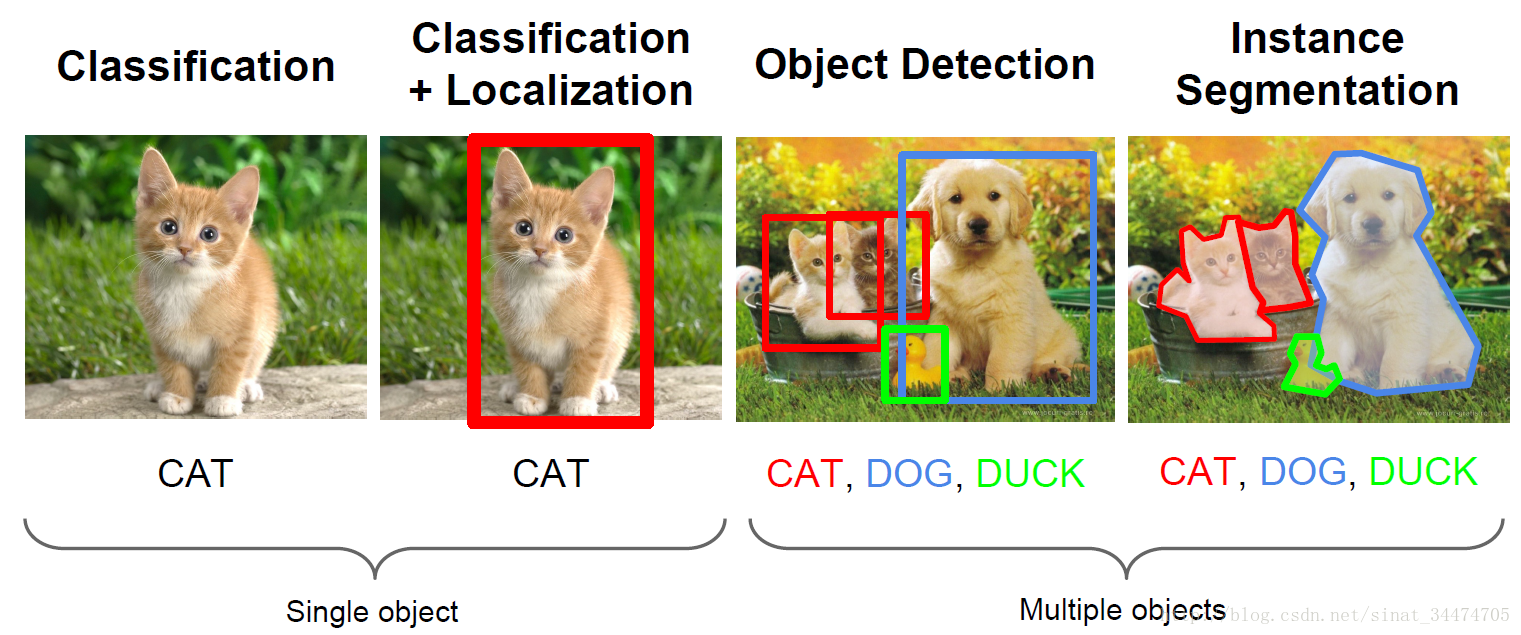
\includegraphics[width=0.9\linewidth]{chapter1_1.png}
  \caption{图形分类、目标定位、目标检测和图像分割的不同\cite{mubiaodingwei}}
  \label{fig:chapter1_1}
\end{figure}

卷积神经网络另一个应用是目标的定位、检测和图像的分割。目标定位的任务是标出图片中物体的位置。目标定位和图像分类都有检测物体类别的属性,它们的不同点是目标定位除了要判别图片中有什么物体之外,还要给出物体在图片中的位置,一般用方框来标记物体位置。
目标检测的任务是识别图片中不定数量物体以及他们各自所在的位置。目标检测与目标定位的不同之处在于目标定位中物体的数量是固定的,而目标检测中物体的数量不是固定的。就是说目标检测需要把图片中所有目标物体全都识别出来并且准确地给出它们的位置。
图像分割的任务是在像素级别圈出图片中的目标物体。图像分割与目标检测不同的地方是图像分割是在像素级别将物体圈出,而目标检测则不需要这么精细,只需要用方框圈出大致的范围即可。如图\ref{fig:chapter1_1}所示,图中用图形展示了图形分类、目标定位、目标检测和图像分割的不同之处。
目标定位和目标检测的典型应用场景是自动驾驶、安全防护和医疗领域。图像分割常用于视频的后期制作和图像处理软件中,如Photoshop、美图秀秀等。

人脸识别技术被广泛应用在移动支付、门禁认证以及考试防作弊等场景。随着人脸识别技术的发展,人脸识别的底层技术也应用到了卷积神经网络。
人脸识别顾名思义就是在图像或视频中识别出人脸的技术。和图像分类技术类似,早期人脸识别技术采用的是传统机器学习的方法。其过程一般是通过摄像头获取图像或视频,然后通过计算机对图片或视频进行预处理,通过选取关键点来提取图片特征,再将提取出来的图片特征与训练好的模型进行比对,从而决定图片的分类。
这种方式虽然在一定程度上可以达到比较理想的效果,可是实际的图片情况是复杂的,比如图片中面部表情不同,光照角度不同,头部姿势不同和遮挡等情况经常出现,这就使得传统的人脸识别技术很难应对。
以卷积神经网络技术为代表的深度学习技术逐渐取代了传统人脸识别的方法,卷积神经网络可以通过学习大量的数据集而找到分类的本质特征,从而达到理想的分类效果。
2014年以DeepFace为代表的利用深度神经网络进行人脸识别的工作相继出现,使得人脸识别准确率不断提高。2015年FaceNet在LFW数据集上达到99.67$\%$的准确率,宣布人工智能首度超过人类的人脸识别能力。随着人脸识别技术的不断成熟,其应用场景也不断增多,如安全防护,金融认证,考试防作弊等,深入到我们日常生活的诸多方面。

卷积神经网络不仅用于图像的处理,其在自然语言处理方面也有出色表现。自然语言处理主要研究人类语言如何快速准确地被计算机系统识别和利用的技术。当今自然语言处理被广泛应用在语言翻译,文章主要观点的概括,语音的辨识等方面。
卷积神经网络由于其出色的特征提取和分类能力,如今也广泛被应用在自然语言处理领域中。

\subsection{选题的意义}
随着卷积神经网络的广泛应用,越来越多的机器学习模型选择卷积神经网络进行学习。与此同时,对机器学习模型的攻击也是层出不穷,用户个人隐私保障的问题急需解决。
随着GDPR的正式施行,用户个人数据的被遗忘权也得到了法律的保护。目前可行的方法是将模型重新训练,可是这样的做法会给企业带来很大的经济负担。
于是研究如何加快基于卷积神经网络的机器学习模型遗忘的算法势在必行。据作者目前了解的情况来看,尚未有一个很成熟的可以大规模使用的基于卷积神经网络的机器学习遗忘算法。
因此,在人们的隐私意识逐步提高的今天,研究基于卷积神经网络的机器学习遗忘算法具有十分重要的现实意义。
\section{研究现状和主要挑战}
机器学习模型遗忘方面的研究从2015年逐渐有学者开始发表论文。刚开始的研究方向是基于一些经典的机器学习算法,比如这篇文章\cite{yinzhicao2015}尝试解决基于贝叶斯推断的遗忘方法,这篇文章\cite{antonio2019}基于k-means聚类算法的遗忘方法等等。
逐渐地,随着欧盟GDPR法规的出台,开始有学者把视线转移到了研究卷积神经网络的遗忘。目前基于卷积神经网络的遗忘仍然是一个开放的问题,尚且没有统一的办法来解决这个问题。

近年来尝试解决卷积神经网络遗忘问题的方法多种多样,例如一种基于网络分割的方法\cite{2019arXiv191203817B},通过将网络分割成若干个小网络,使得重新训练的任务量从整个大网络减小成每个小网络重新训练的工作量。
这样的方法虽然在重新训练时间上面有所降低,同时也带来需要将所有网络预测结果进行综合的额外工作量,使得网络在进行预测时效率有所降低。
还有一种思路是基于正则化和增加噪音的方法,这个方法\cite{Golatkar_2020_CVPR}通过重新设计损失函数并且在权重上增加随机噪音的方法实现遗忘效果。
这种方法能达到很迅速遗忘的效果,可是增加噪声会不可避免地减少没被遗忘类别的准确率。总之到目前为止,尚没有一种方法取得了压倒性的优势,因此基于卷积神经网络的遗忘问题仍然是开放的。

基于卷积神经网络的遗忘问题之所以这么困难是因为卷积神经网络的非线性特征,这种非线性特征使得人们很难寻找其参数更新的规律,换句话说就是可解释性很差。在输入多个训练数据参与训练之后,我们无法通过反向还原的方法通过数学计算将网络还原到训练之前的那个状态。
虽然卷积神经网络的优点有很多,可是卷积神经网络现在对人类来说仍然是一个黑箱,无法寻找到卷积神经网络参数更新的规律。因此,寻找如何更新参数的方法就是本研究方向的一个挑战。

另外,卷积神经网络模型利用遗忘算法遗忘过后,如何评价遗忘的效果也是这个研究方向的一个挑战。我们的一个直觉是通过测试的准确率来评价遗忘效果。经过分析后发现,这个指标仅能作为一个辅助指标进行参考。
因为遗忘问题的本质并不是遗忘得越彻底越好,如果通过掩盖的方法来降低遗忘类别的准确率反而能够给攻击者可乘之机。因为攻击者可以利用成员推断攻击来判断一个训练数据是否曾经被用于网络模型的训练,这种情况往往也不是用户期待发生的事情。这种情况可以被一个词很好的描述,“欲盖弥彰”。
因此,如何评价网络模型已经达到了一个理想的遗忘效果也是本文的一个挑战。

\section{主要的研究方法}
为了解决卷积神经网络的遗忘问题,在本文中我们利用了卷积神经网络的一个重要特性,即分层抽象特性。在卷积神经网络中,一个个卷积核就是特征的提取器,在不同的网络层次中,这些提取器对特征提取的分工是各不相同的。
较低层次的特征提取器会提取一些基本特征,比如图像的不同方向的直线特征。随着网络层次的提高,特征提取器会提取一些较为抽象的特征。我们在后续实验中也验证了这一特性。我们正是利用了这一特性,提出了一种更新网络参数的策略,那就是只更新和最终分类相关的较高层次的网络参数,随后再利用保留集训练网络,直至网络收敛。
那么有人不禁会问,这样是否会达到理想的遗忘效果。我们通过一些参考指标对网络的遗忘效果进行评估后发现,这种方法可以不用更新全部网络参数就可以达到理想的遗忘效果,而且遗忘时间也较完全重新训练全部网络具有竞争力。总结以上,本文的贡献可以分为以下几个方面:

第一,本文基于卷积神经网络的分层抽象特性,提出了一种更新网络参数的方法。经实验证明这种方法可以达到很好的遗忘效果,而且在遗忘时间方面对比完全重新训练网络具有一定的竞争优势。

第二,经过实验表明,本文提出的方法具有遗忘的连续性,适用于多次遗忘操作。因此本文所使用的方法具有广泛应用的前景。

第三,本文提出了将卷积神经网络的分层抽象特性用于解决遗忘问题的思路。

\section{论文结构安排}
第一章是引言,首先介绍本文的研究背景和选题意义,然后介绍机器学习遗忘面临的主要挑战和发展现状。然后简要说明了本文中所用到的解决问题的思路和方法,提出了本文的主要贡献。
第二章中首先介绍了迁移学习和增量学习的研究领域和网络参数共享方向的研究成果。然后介绍了机器学习遗忘的相关研究工作,主要涉及到非卷积神经网络的遗忘,和基于卷积神经网络的遗忘学习算法。
第三章是本文的核心章节,首先介绍了卷积神经网络的基本原理与本文解决遗忘问题的思路来源,即卷积神经网络的分层抽象特性。然后分步骤具体介绍了遗忘问题的解决方案。最后介绍了评价遗忘效果的三个指标。
第四章是实验验证,介绍了本文实验所用的环境和实验方法的设计,最后展示了实验结果。
第五章是全文的总结,首先总结了各个章节的主要内容,然后讲了本文的一些不足之处,最后对基于卷积神经网络的遗忘方法可能的发展方向进行了展望。
\section{本章小结}
本章提出了本文的研究背景、研究意义和研究现状,然后又简要说明了本文遇到的主要挑战和解决问题的主要思路。最后对论文的结构安排做了总体性的概括。
